\section{Methodology}

This section discusses the geometry and the modeling approach in this paper.
The reactor model geometry in this paper is kept unchanged from the models
used by Fiorina et al. \cite{fiorina_modelling_2014} and Aufiero et al.
\cite{aufiero_development_2014}, henceforth referred to as the
Polimi/TUDelft models, to provide a fair comparison in this
benchmarking exercise.

\subsection{Reactor Model Geometry and Group Constant Generation}

For this work, we used the reference square-cylindrical \gls{MSFR} design to
benchmark Moltres against results published by Fiorina et al. and Aufiero et
al. It is a 2-D axisymmetric design with the sixteen individual external loops
homogenized into a single outer loop as shown in Fig. \ref{fig:msfrgeom}. For
the multi-group
cross sections and group constants calculations in Serpent, we extended this
2-D axisymmetric model into a 3-D model by a simple full rotation about the
central axis. The material definitions are the same as those specified in the
reference \gls{MSFR} model. Accordingly, the pump and heat exchanger regions
are assumed to be composed of 100\% fuel salt. While this may not be entirely
accurate, the exact details of the pump and heat exchanger systems are still
be researched, and this external loop region is presumed to be of little
neutronic importance due to its position behind the strong boron carbide
neutron absorber layer.
%
\begin{figure}[htb!] 
	\centering
	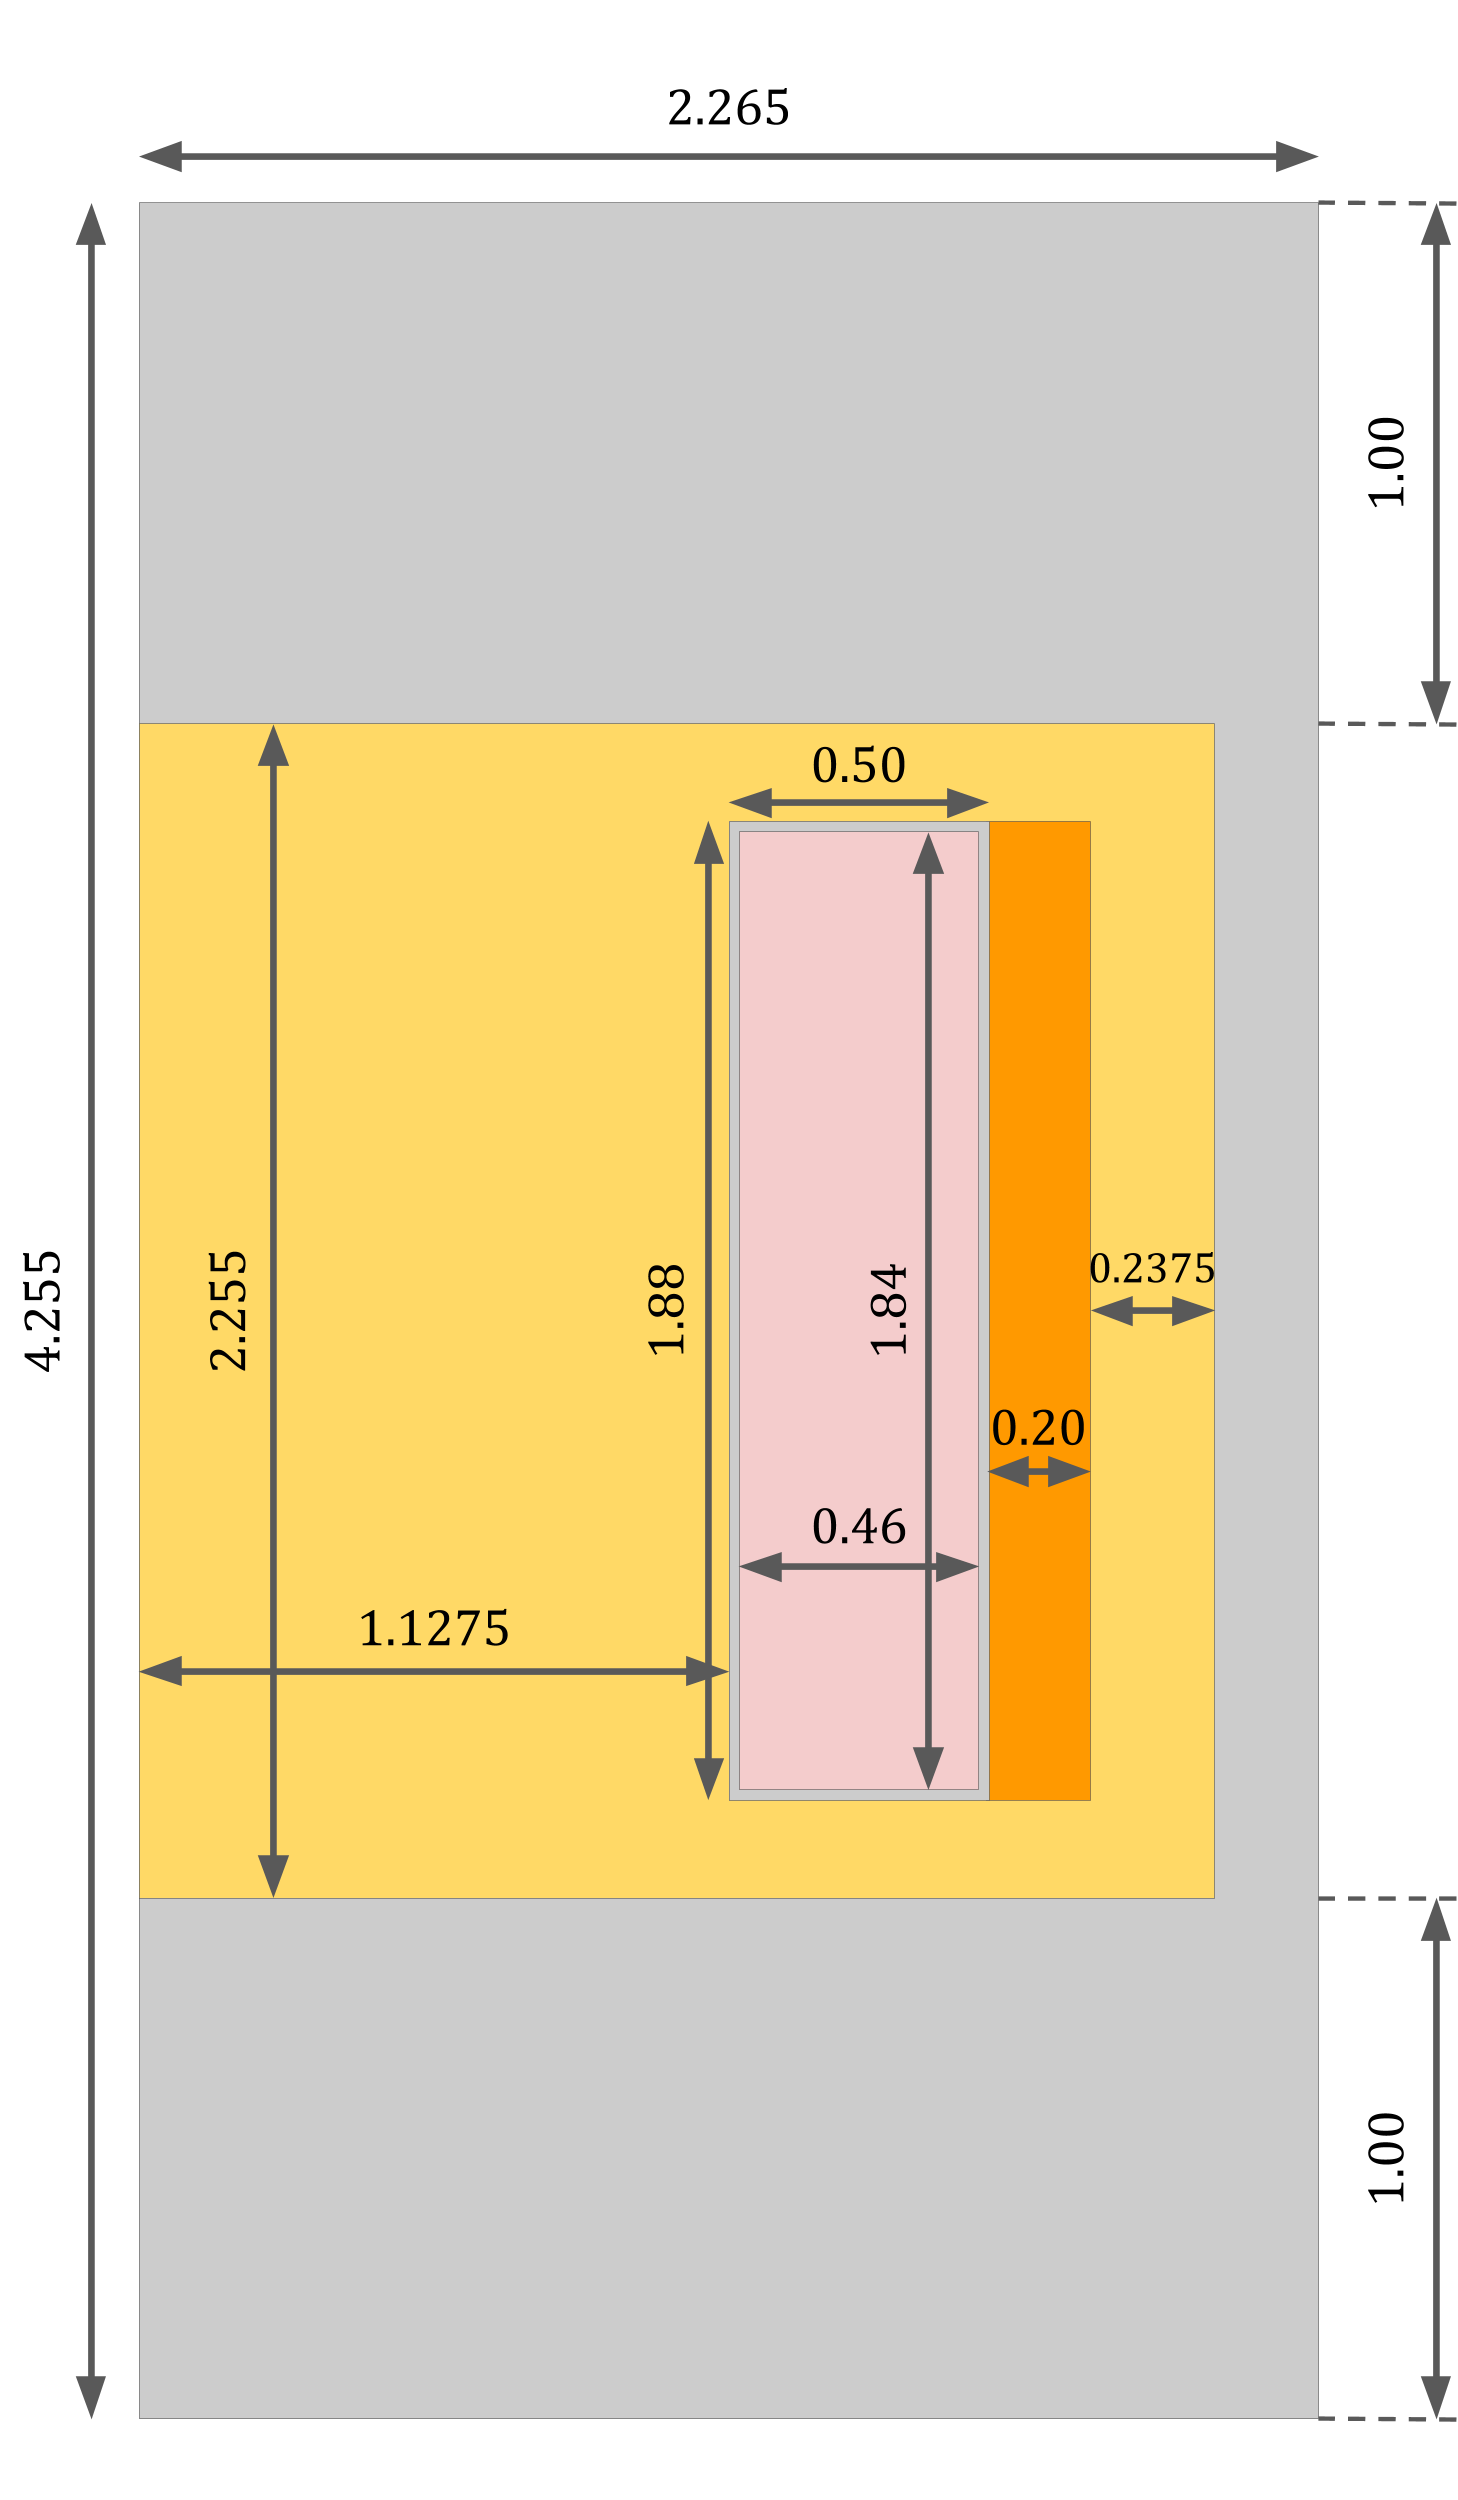
\includegraphics[width=0.5\textwidth]{msfr-geom}
	\caption{2-D axisymmetric model of the \gls{MSFR} core used for the
	simulations in Serpent and Moltres. All dimensions are in meters.
	\cite{brovchenko_neutronic_2019}}
	\label{fig:msfrgeom}
\end{figure}

There are two key differences between our \gls{MSFR} model geometry in
Moltres and the Polimi/TUDelft models. The first difference is a relative
minor change to the mesh by the exclusion of the 2 cm thick structural
material around the blanket tank that separates the fuel and blanket salts.
We removed this feature in our finite element mesh as we had difficulty
meshing this layer that is relatively much thinner than the rest of the model.
Any impact on the
neutron flux is expected to be minimal. Furthermore, we solved for the
temperature distribution only in the primary loop and applied homogeneous
Neumann boundary conditions for temperature on the core walls, as was done in
the Polimi/TUDelft models. Therefore, we believe the overall impact on the
results is negligible.

The second difference pertains to the modeling of the external loop. In its
current implementation, Moltres lacks pump- and heat exchanger-equivalents in
the code. Thus, the external loop is modeled as a 1-D pipe with a point heat
sink to represent the heat exchanger. Instead of pumps, the flow is driven by
Dirichlet boundary conditions for velocity on the inlet and outlet boundaries
of the 2-D axisymmetric central core geometry and the 1-D external pipe
geometry. All flow-dependent variables such as temperature, \glspl{DNP}, and
decay heat precursors are fully conserved as they loop around between the two
regions. As a result, this approach shares some similarities with the
geometric multiscale modeling approach by Zanetti et al.
\cite{zanetti_geometric_2015} Future models could
create a better representation of the primary loop by implementing a whole
continuous loop with pressure increases and drops corresponding to the pumps
and heat exchangers. 

We used the JEFF-3.1.2 cross-section library \cite{oecd/nea_jeff-3.1.2_2014}
for group constant generation in
Serpent. We set a neutron population of 200,000 neutrons per cycle with 50
inactive and 500 active cycles for a total of 100 million neutron histories.
The material compositions of the various reactor components follows the
benchmark specification, with slight adjustments to the
ratio of $^{232}$Th to $^{233}$U to obtain $k_{\text{eff}}=1$ at 973 K. The
resulting mole fraction is very close to a result cited in the neutronics
benchmark paper which was also generated from Serpent using the JEFF-3.1.1
library (Table \ref{table:mole}). The differences can be largely attributed to
the statistical uncertainty for both results. We divided the primary loop into
3 subdivisions: core, inlet/outlet, and heat pump/exchanger regions. This was
motivated by the difference in neutronic importance of those regions. We
followed the same six-group
structure (Table \ref{table:bound}) as the Polimi COMSOL model
\cite{fiorina_modelling_2014}. The
energy boundaries for the six neutron energy groups are shown in Table
\ref{table:bound}. For the \glspl{DNP}, the JEFF-3.1.2 library provides
eight pre-defined \gls{DNP} groups based on their half-lives. The relevant
group constants for Moltres simulations are: the various macroscopic neutron
cross-sections, neutron diffusion coefficient, average fission energy, average
neutron yield, inverse neutron speed, fission spectrum, \gls{DNP} group
constants, and effective delayed neutron fractions.

Moltres, by extension from MOOSE, accepts various mesh file formats; we refer
readers to the MOOSE framework website for the full list of supported file
formats. We used the Trelis 16.5 \cite{noauthor_trelis_2018} to generate the
\gls{MSFR} mesh (Fig. \ref{fig:msfrgeom}) in this work. There are finer mesh
elements around the absorber region boundaries to accurately capture the steep
drop in neutron flux at those boundaries.
%
\begin{table}[htb!]
	\centering
    \caption{Comparison of mole fractions and $k_{\text{eff}}$ uncertainty
    of $^{232}$Th and $^{233}$U in
    the fuel salt composition adjusted for $k_{eff}=1$ at 973 K.}
\begin{tabular}{l S S}
	\hline
	\textbf{Property} & \textbf{This paper} & \textbf{Benchmark
	\cite{brovchenko_neutronic_2019}} \\
	\hline
    $^{232}$Th mol\% & 19.943 \% & 19.948 \% \\
    $^{233}$U mol\% & 2.557 \% & 2.551 \% \\
    $k_{\text{eff}}$ uncertainty & 4.9 pcm & 4.6 pcm \\
    \hline
\end{tabular}
\label{table:mole}
\end{table}
%
\begin{table}[htb!]
	\centering
	\caption{Neutron energy group upper bounds used in Serpent.}
	\begin{tabular}{c S}
		\hline
		{Group number} & {Upper bound [MeV]}\\
		\hline
		1 & 7.485$\times 10^{-4}$\\
		2 & 5.5308$\times 10^{-3}$\\
		3 & 2.47875$\times 10^{-2}$\\
		4 & 0.4979\\
		5 & 2.2313\\
		6 & 12\\
		\hline
	\end{tabular}
	\label{table:bound}
\end{table}
%
\subsection{Modeling Approach}

Moltres is an application built on the MOOSE \cite{gaston_physics-based_2015}
framework. MOOSE provides a simplified interface for developing fully
coupled multiphysics solvers while leveraging on sophisticated computational
tools: PETSc \cite{satish_petsc_2019}, a non-linear solver package, and
libMesh \cite{kirk_libmesh:_2006}, a finite element library. In Moltres, the
various physical phenomena described by each term in the \glspl{PDE} are
represented by ``kernels'' and boundary conditions. For
example, the individual terms for neutron diffusion, removal, scattering, etc.
each have their own representative kernel. Kernels provide weak
form representations in MOOSE through the calculation of residual and Jacobian
contributions of the corresponding physics. Multiple kernels from the same
\gls{PDE} may also be grouped together for ease of implementation. The neutron
flux and velocity variables were approximated by first-order
Lagrangian finite element shape functions, while the \gls{DNP} and decay heat
precusor variables were approximated by constant monomial shape functions.

\subsubsection{Neutronics}

The neutronics is implemented through the deterministic multi-group neutron
diffusion equations. Due to its modular structure, Moltres can solve for an
arbitrary number of neutron and \gls{DNP} group. Moltres requires group
constant data from dedicated neutron transport codes such as Serpent or SCALE
\cite{dehart_reactor_2011}, and there are python scripts available on the
Moltres GitHub repository \cite{lindsay_moltres_2017} to convert the
Serpent/SCALE output file into a Moltres-compatible format.

The governing equation for time-dependent multi-group neutron diffusion in
Moltres is:
%
\begin{align}
	\frac{1}{v_g} &\frac{\partial \phi_g}{\partial t} - \nabla \cdot D_g
	\nabla \phi_g + \Sigma^r_g \phi_g \nonumber \\ 
	&= \sum^G_{g \neq g'} \Sigma^s_{g' \rightarrow g} \phi_{g'} + \chi^p_g
	\sum^G_{g'=1} (1-\beta) \nu \Sigma^f_{g'} \phi_{g'} + \chi^d_g \sum^I_i
	\lambda_i C_i. \label{eq1}
\end{align}
%	\intertext{where}
%	v_g &= \text{average speed of neutrons in group }g \nonumber \\
%	\phi_g &= \text{flux of neutrons in group }g \nonumber \\
%	t &= \text{time} \nonumber \\
%	D_g &= \text{diffusion coefficient of neutrons in group }g \nonumber \\
%	\Sigma^R_g &= \text{macroscopic cross-section for removal of neutrons} 
%	\nonumber \\
%	&\text{from group }g \nonumber \\
%	\Sigma^s_{g' \rightarrow g} &= \text{macroscopic cross-section of
%	scattering from }g' \text{ to }g \nonumber \\
%	\chi^p_g &= \text{prompt fission spectrum neutrons in group }g \nonumber
%	\\
%	G &= \text{number of discrete neutron groups, }g \nonumber \\
%	\nu &= \text{average number of neutrons produced per fission} \nonumber \\
%	\Sigma^f_{g} &= \text{macroscopic fission cross-section} \nonumber \\
%	&\text{for neutron in group }g \nonumber \\
%	\chi^d_g &= \text{delayed fission spectrum neutrons in group }g \nonumber
%	\\
%	I &= \text{number of delayed neutron precursor groups} \nonumber \\
%	\beta &= \text{delayed neutron fraction} \nonumber \\
%	\lambda_i &= \text{average decay constant of delayed neutron} \nonumber \\
%	&\text{precursors in precursor group }i \nonumber \\
%	C_i &= \text{concentration of delayed neutron precursors} \nonumber \\
%	&\text{in precursor group }i. \nonumber
%\end{align}

We used six energy groups with the cross sections generated on Serpent for
temperatures from 900 K to 1200 K at 50 K intervals. Moltres contains various
interpolation methods for the cross sections for temperatures that fall
between the given temperatures; we applied the spline method for this work.
The temperature dependence of the cross sections from Serpent encompasses both
the Doppler effect and density dependence. We assumed vacuum boundary
conditions for all six neutron groups along the external boundaries of the
geometry and homogeneous Neumann boundary conditions along the axial boundary.

The \glspl{DNP} are governed by the following equation:
%
\begin{align}
	\frac{\partial C_i}{\partial t} = - \nabla(\overrightarrow{u} C_i)
	+ \nabla \cdot \frac{\mu_T}{\rho Sc_T} \nabla C_i	
	- \lambda_i C_i + \sum^G_{g'=1} \beta_i \nu \Sigma^f_{g'}
	\phi_{g'}. \label{eq2}
\end{align}

There are eight \gls{DNP} groups with decay constants pre-defined by the
JEFF-3.1.2 library \cite{oecd/nea_jeff-3.1.2_2014}. Similar to the
Polimi/TUDelft models, the \gls{DNP} equation (Eq. \ref{eq2}) contains both
convective and diffusive terms. The diffusive term arises from turbulent
diffusion approximated by the turbulent viscosity, and the turbulent Schmidt
number assumed to be 0.85. The turbulent viscosity is discussed in greater
detail in the thermal-hydraulics subsection. The \glspl{DNP} are simulated
only in the central core region and the 1-D pipe representing the external
loop. Homogeneous Neumann boundary conditions were applied along the walls of
the central core region, and inflow and outflow boundary conditions were
applied on the inlet and outlet boundaries respectively. We used a prescribed
velocity value in the 1-D external loop region to simulate the time that the
precusors spend outside of the core.

We also included a decay heat model based on a previous work
\cite{aufiero_extended_2013} on the \gls{MSFR}, which found that using three
decay heat precursor groups could model decay heat in the \gls{MSFR} for up to
300 seconds after a full shutdown with less than 2 \% relative error
\cite{aufiero_development_2014}. The decay heat parameters are shown in Table
\ref{table:decay}, and the equation describing the behavior of decay heat
precursors is given as:
%
\begin{align}
	\frac{\partial D_i}{\partial t} = - \nabla(\overrightarrow{u} D_i)
	+ \nabla \cdot \frac{\mu_T}{\rho Sc_T} \nabla D_i	
	- \lambda_i D_i + \sum^G_{g'=1} f_i \nu \Sigma^f_{g'}
	\phi_{g'}. \label{eq2}
\end{align}

\begin{table}[htb!]
	\centering
	\caption{Decay heat group parameters \cite{fiorina_modelling_2014}.
	$\lambda_i$ and $f_i$ are the decay constants and decay heat fractions
	associated to group $i$.}
	\begin{tabular}{S S S}
		\hline
		{Decay heat group} & {$\lambda_i$ [s$^{-1}$]} & {$f_i$} \\
		\hline
		1 & 0.1974 & 0.0117 \\
		2 & 0.0168 & 0.0129 \\
		3 & 3.58 $\times 10^{-4}$ & 0.0186 \\
		\hline
	\end{tabular}
	\label{table:decay}
\end{table}

\subsubsection{Thermal-hydraulics}

The thermal-hydraulics is modeled based on the incompressible Navier-Stokes
equations with the Boussinesq hypothesis for eddy viscosity. Most of the
Navier-Stokes module in Moltres is derived from the MOOSE Navier-Stokes module
\cite{peterson_overview_2017}. In addition to the intrinsic material dynamic
viscosity, we introduced an eddy viscosity term to approximate turbulent flow
effects. The current implementation of Moltres does not have a turbulence
model such as the \gls{RANS} equations used in the Polimi/TUDelft models.
Thus, we made a zeroth-order approximation of the eddy viscosity based on the
results reported in the Polimi/TUDelft models.

The flow rate is dictated by the inflow boundary condition at the core inlet
to meet the 4.5 m$^3$ s$^{-1}$ specification. We imposed no-slip boundary
conditions on the walls of the core, and homogeneous Neumann boundary
conditions on the core outlet. The energy balance equation for temperature is
given in Eq. *. The diffusion term includes turbulent heat diffusivity based
on the eddy viscosity and the turbulent Prandtl number, which we assume to be
0.85.
